\begin{frame}[t]
    \titlepage
\end{frame}

\begin{frame}{Motivation}
\begin{center}
\begin{figure}
   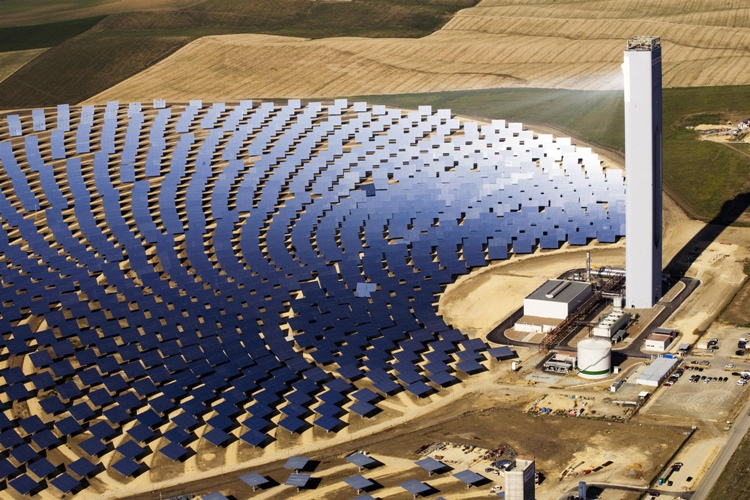
\includegraphics[width=0.6\paperwidth, trim=0pt 80pt 0pt 0pt, clip]{./figs/solartower}
   \caption{Solar tower power plant. Heliostats reflect onto a receiver in order to heat up a medium for energy conversion.}
\end{figure}
\end{center}
Sun's position changes continuously, thus for effective energy conversion we need to rotate the heliostats. \\
\hspace{1cm}$\Rightarrow$ each heliostat requires a data and power cable
\end{frame}

\begin{frame}\frametitle{Problem}
\begin{itemize}
  \item Consider a complete and undirected graph $G=(V,E)$ with $V:=\{T\} \cup V_H$, where $T$ is the designated solar tower and $V_H$ is the set of heliostats.
  
  \visible<2->{\vspace*{0.3cm}
  \item Goal: Find subgraphs $H_{\text{data}},H_{\text{power}}\subseteq G$ with minimal total costs that both connect all heliostats with the solar tower.
    \begin{itemize}
      \item data cable: cable and switch costs
      \item power cable: cable costs
    \end{itemize}
  }
  
  \visible<3->{\vspace*{0.2cm}\item Constraints:
  \begin{itemize}
    \item no intersecting edges
    \item cables have capacity and length constraints
    \item switches limit connectivity at heliostats for data cables
  \end{itemize}
  }
\end{itemize}
\end{frame}

\begin{frame}\frametitle{Problem: Data cable}
\begin{table}
  \caption{Data cables with their limitations and costs. We can only connect two heliostats with a copper cable.}
  \begin{tabular}{l|cc|c}
    Cable & Max. capacity & Max. length [m] & Price [\euro/m] \\
    \toprule
    Copper & 2 & 100 & 0.7 \\
    Fiberglass & - & - & 2
  \end{tabular}
\end{table}
\visible<2->{
  \begin{table}
    \caption{Switch prices, for 8-/16-port switches we can either use copper or fiber-glass output. Endpoints are only used for copper cables.}
    \begin{tabular}{l|cc}
      Switch & Max. degree & Price [\euro/p. piece] \\
      \toprule
      Endpoint & 1 & 10 \\
      Conductor & 2 & 100 \\
      8-port copper/fiberglass switch & 9 & 800 \\
      16-port copper/fiberglass switch & 17 & 1500
    \end{tabular}
  \end{table}
}
\end{frame}

\begin{frame}\frametitle{Problem: Power cable}
\begin{table}
  \caption{Power cables with their connectivity limitations and prices.}
  \begin{tabular}{l|cc|c}
    Cable & Max. capacity & Max. length [m] & Price [\euro/m] \\
    \toprule
    NYY-J 3x2.5 RE & 56 & 38.36 & 0.58 \\
    NYY-J 3x4 RE & 73 & 47.08 & 0.87 \\
    NYY-J 3x6 RE & 92 & 56.04 & 1.24 \\
    NYY-J 3x10 RE & 124 & 69.30 & 1.95 \\
    NYY-J 3x16 RE & 162 & 84.87 & 3.13 \\
    \midrule
    NYY-J 3x25 RM & 209 & 102.79 & 5.19 \\
    NYY-J 3x35 RM & 250 & 120.31 & 6.90
  \end{tabular}
\end{table}
\begin{itemize}
  \item For instances with more than 250 heliostats we need to use more than one outgoing cable from the solar tower \\ $\Rightarrow$ Partitioning problem
\end{itemize}
\end{frame}

\begin{frame}\frametitle{Problem: Installation cost}
\begin{table}
  \caption{Depending on the location we have different installation costs for trenches and working power.}
  \begin{tabular}{l|c}
    Country & Price [\euro/m] \\
    \toprule
    Australia & 50 \\
    Spain & 25 \\
    South Africa (RSA) & 10 \\
    United Arab Emirates (UAE) & 10
  \end{tabular}
\end{table}
\begin{itemize}
  \item additionally: protective foil (+2\euro/m)
\end{itemize}
Thus for a meter of glasfiber in Australia we need to pay
\begin{tabular}{rl}
  \phantom{+}50\euro & installation cost \\
  +2\euro & glasfiber cable \\
  +2\euro & protective foil \\
  \cmidrule{0-1} \\
  54\euro
\end{tabular}
\end{frame}

\begin{frame}[t]{Our approach}
\vfill
\begin{itemize}
  \item Consider a precomputed partioning $\Rightarrow$ eases capacity constraint and computation time
  \item Focus on data cabling due to high switch costs
  \begin{itemize}
    \item compute solution only on data cable
    \item afterwards compute power cable assignment greedily with data cable solution
  \end{itemize}
  \end{itemize}
$\Rightarrow$ consider solution that installs data and power cable together in trenches, that is, we only have one subgraph $H\subseteq G$
\vfill
\end{frame}

%\begin{frame}[t]{Initial solutions}
%\centering
%\begin{tikzpicture}[scale = 1.5,sibling distance=8em,
%  every node/.style = {shape=rectangle, rounded corners,
%    draw, align=center,
%    top color=white, bottom color=white}]]
%  \node {Cost factors}
%    child { node {Switches} 
%        child { node(e1) {Hamiltonian paths} } }
%    child { node {Cable meters}
%		child { node(e2) {MST} } 
%		};
%\begin{scope} [shift={(0cm,-4.5cm)}]
%\node(e3) {Lazy-Branching};  
%\end{scope}
%\begin{scope}[dashed] 
%\draw (e1)--(e3); 
%\draw (e2)--(e3); 
%\end{scope}
%\end{tikzpicture}
%\end{frame}